
%-------------------------------------------------------------------------
\vspace{0.2cm}
\section{Experiment}
\label{sec:experiment}
In this section, we first introduce our adopted dataset and implementation settings. Then, we conduct a series of experiments with detailed ablation studies to show the effectiveness of our approach.

\subsection{Experimental Settings}
% \KY{which dataset do we use for ablation study? name this here.}
\paragraph{Dataset and Metrics.}
We evaluate our TiG-BEV on nuScenes dataset\cite{b6}, which is one of the most popular large-scale outdoor public datasets for autonomous driving. It consists of 700, 150, 150 scenes for training, validation and testing, respectively. It provides synced data captured from a 32-beam LiDAR at 20Hz and six cameras covering 360-degree horizontally at 12Hz. We adopt the official evaluation toolbox provided by nuScenes, which reports the nuScenes Detection Score (NDS) and mean Average Precision (mAP), along with mean Average Translation Error (mATE), mean Average Scale Error (mASE), mean Average Orientation Error (mAOE), mean Average Velocity Error (mAVE), and mean Average Attribute Error (mAAE).

\begin{table}[t!]
\centering
\caption{\textbf{Performance Comparison without CBGS Strategy~\cite{b56}.} For all methods, we adopt ResNet-101 as the 2D backbone and $512\times 1408$ as the image resolution. * denotes our implementation.}
%\vspace{-2mm}
%\resizebox{1\columnwidth}{!}
\resizebox{1\columnwidth}{!}
%{\tablestyle{5pt}{1.2}
{\tablestyle{10pt}{1}
\begin{tabular}{c|cc}
\toprule[1.2pt]
          Method& mAP&NDS  \\
          \midrule
          % CenterPoint&  0.564 & 0.646 \\ %得有换行双斜杠
          % \midrule
          BEVDet$^*$& 0.272 & 0.297 \\
          \rowcolor{gray!12}\textbf{+ TiG-BEV}& \textbf{0.375 (\textcolor{blue}{+10.3\%})} &\textbf{0.388 (\textcolor{blue}{+9.1\%})} \\\midrule
          %\rowcolor{gray!12}&   \textbf{}&\textbf{}\\\midrule
          BEVDet4D$^*$& 0.336 & 0.435 \\
          \rowcolor{gray!12}\textbf{+ TiG-BEV}& \textbf{0.409 (\textcolor{blue}{+7.3\%})} &\textbf{0.489 (\textcolor{blue}{+5.4\%})} \\\midrule
          %\rowcolor{gray!12}&   &\\\midrule
          %BEVDepth& 0.345 & 0.366 \\
          %\rowcolor{gray!12}\textbf{+ TiG-BEV}& \textbf{0.403} &\textbf{0.416} \\
          %\rowcolor{gray!12}&   \textcolor{blue}{+5.8\%}&\textcolor{blue}{+5.0\%}\\
          BEVDepth$^*$& 0.393 & 0.487 \\ 
          \rowcolor{gray!12}\textbf{+ TiG-BEV}& \textbf{0.430 (\textcolor{blue}{+3.7\%})} &\textbf{0.514 (\textcolor{blue}{+2.7\%})} \\
          %\rowcolor{gray!12}&   &\\
    \bottomrule[1.2pt]
    \end{tabular}}
    \label{tab:aaaa}
    %\vspace{-5mm}
\end{table}
\begin{table}[t!]
\centering
    \caption{\textbf{Comparison with BEVDistill~\cite{b9}.} $\dagger$ and * denote the implementation of BEVDistill and ours, respectively. We present the performance improvement of the learning methods correspondingly to their implemented baselines.}
    %\vspace{-2mm}
    \resizebox{1\columnwidth}{!}
    {\tablestyle{10pt}{1.0}
    \begin{tabular}{c|cc}
    \toprule[1.2pt]
          Method&mAP&NDS  \\
          \midrule
          BEVDepth$\dagger$ &0.311       &  0.432     \\
          \rowcolor{gray!12}BEVDepth$^*$ &0.329       &  0.431     \\
          \midrule
          + BEVDistill &0.332 (\textcolor{blue}{+2.1\%})       &  0.454 (\textcolor{blue}{+2.2\%})     \\
          %&\textcolor{blue}{+2.1\%} &\\
          \rowcolor{gray!12}\textbf{+ TiG-BEV} &\textbf{0.366 (\textcolor{blue}{+3.7\%})}       &  \textbf{0.461 (\textcolor{blue}{+3.0\%})}     \\ 
          %\rowcolor{gray!12}&\textbf{} &\textbf{}\\
    \bottomrule[1.2pt]
    \end{tabular}}
    \label{cccc}
    %\vspace{-5mm}
\end{table}
\begin{figure*}[ht]
% \vspace{-0.5cm}
    \centering
    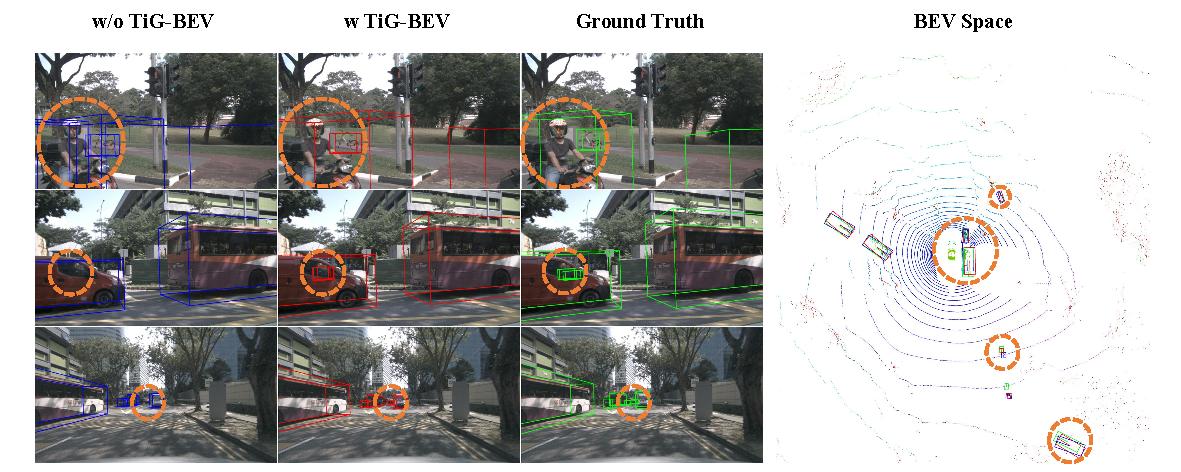
\includegraphics[scale=0.85]{cvpr_2022/det_result.pdf}
    \caption{\textbf{Visualization of Detection Results}. From left to right, we show the 3D object detection before and after the TiG-BEV learning schemes, ground-truth annotations, along with the overall BEV-space results.
    }
    \label{fig:aabb}
    %\hspace{-5cm}
\end{figure*}
\paragraph{Implementation Details.}
We implement our TiG-BEV using the BEVDet\cite{b19,b23} code base on 8 NVIDIA A100 GPUs, which is built on MMDetection3D toolkit\cite{b55}. A pre-trained CenterPoint~\cite{b53} with voxel size of $[0.1,0.1,0.2]$ is adopted as the LiDAR-based teacher, and the camera-based students include BEVDepth~\cite{b7}, BEVDet~\cite{b19} and BEVDet4D~\cite{b23}. During inference, the camare-based detecots only take multi-view images as input without the LiDAR data or teachers.
Referring to BEVDepth, we additionally add the dense depth supervision on top of BEVDet and BEVDet4D besides our TiG-BEV. We follow their official training configurations and hyperparameters as default, including data augmentation (random flip, scale and rotation), training schedule (2x), and others (AdamW optimizer~\cite{b16}, 2e-4 learning rate and batch size 8). For the main results on nuScenes val set in Table~\ref{tab:nus_val_sota}, we compare our TiG-BEV with all other methods under the CBGS strategy~\cite{b56}. For all other results, we do not utilize CBGS to better reveal the significance of proposed methods.

% Our TiG-BEV is trained for 2 × schedule 

% (20 epochs with CBGS strategy\cite{b56} or 24 epochs without CBGS strategy) with a batch size of 8 on 8 NVIDIA A100 GPUs. We use AdamW\cite{b16} optimizer with the initial learning rate of 2e-4, which drops at epoch 19 and 23 by a factor of 0.1 without CBGS strategy and drops at epoch 16 and 19 by a factor of 0.1 with CBGS strategy. In terms of data augmentation, the input images and points are randomly flipped, scaled and rotated. For the purpose of fair comparison, the above settings are aligned with mainstream methods. In ablation studies, we use BEVDepth\cite{b23} without CBGS strategy as our baseline.
%When we compare with other methods, we use BEVDet4d\cite{b23} with absolute depth supervision and CBGS strategy as our baseline. Otherwise, the results shown in tables, such as ablation studies, are taken from experiments without CBGS strategy.
%\begin{table}
% \vspace{-1.1cm}
\small
\centering

\begin{tabular}{L{4.0cm}|C{1.5cm}|C{1.5cm}|C{1.5cm}|C{1.5cm}}
\hline

\hline

\hline
Method  & Params  &FLOPs & Top1 & Latency\\
\hline

\hline
\hline
MobileNetV3-Small~\cite{howard2019searching}  & 2.9M & 0.1G & 67.4 & \textbf{5ms} \\
SeaFormer-T  & 1.8M & 0.1G & 67.9 & 7ms \\
\textbf{SeaFormer-T++}  & 1.9M & 0.1G & \textbf{69.8} & 7ms \\
\hline

\hline
\hline
MobileViT-XXS~\cite{mehta2021mobilevit}  & 1.3M & 0.4G & 69.0 & 24ms \\
MobileViTv2-0.50~\cite{mehta2022separable} & 1.4M & 0.5G & 70.2 & 32ms \\
MobileOne-S0*~\cite{vasu2022improved} & 2.1M & 0.3G & 71.4 & 14ms \\
MobileNetV2~\cite{sandler2018mobilenetv2} & 3.4M & 0.3G & 72.0 & 17ms \\
Mobile-Former96~\cite{chen2022mobile} & 4.8M & 0.1G & 72.8 & 31ms \\
SeaFormer-S & 4.1M & 0.2G & 73.3 & 12ms \\
\textbf{SeaFormer-S++} & 4.2M & 0.2G & \textbf{74.5} & \textbf{12ms} \\
\hline

\hline
\hline
EdgeViT-XXS~\cite{pan2022edgevits} & 4.1M & 0.6G & 74.4  & 71ms \\
LVT~\cite{yang2022lite} & 5.5M & 0.9G & 74.8 & 97ms \\
MobileViT-XS~\cite{mehta2021mobilevit} & 2.3M & 0.9G & 74.8 & 54ms \\
MobileNetV3-Large~\cite{howard2019searching} & 5.4M & 0.2G & 75.2 & \textbf{16ms} \\
Mobile-Former151~\cite{chen2022mobile} & 7.7M & 0.2G & 75.2 & 42ms \\
MobileViTv2-0.75~\cite{mehta2022separable} & 2.9M & 1.0G & 75.6 & 68ms \\
MobileOne-S1*~\cite{vasu2022improved} & 4.8M & 0.8G & 75.9 & 40ms \\
SeaFormer-B & 8.7M & 0.3G & 76.0 & 20ms \\
\textbf{SeaFormer-B++} & 8.8M & 0.3G & \textbf{77.0} & 20ms \\
\hline

\hline
\hline
MobileOne-S2*~\cite{vasu2022improved} & 7.8M & 1.3G & 77.4 & 63ms \\
EdgeViT-XS~\cite{pan2022edgevits} & 6.8M & 1.1G & 77.5  & 124ms \\
MobileViTv2-1.00~\cite{mehta2022separable} & 4.9M & 1.8G & 78.1 & 115ms \\
MobileOne-S3*~\cite{vasu2022improved} & 10.1M & 1.9G & 78.1 & 91ms \\
MobileViT-S~\cite{mehta2021mobilevit} & 5.6M & 1.8G & 78.4 & 88ms \\
EfficientNet-B1~\cite{tan2019efficientnet} & 7.8M & 0.7G & 79.1 & 61ms \\
EfficientFormer-L1~\cite{li2022efficientformer} & 12.3M & 1.3G & 79.2 & 94ms \\
Mobile-Former508~\cite{chen2022mobile}  & 14.8M & 0.5G & 79.3 & 102ms \\
MobileOne-S4*~\cite{vasu2022improved} & 14.8M & 3.0G & 79.4 & 143ms \\
SeaFormer-L & 14.0M & 1.2G & 79.9 & 61ms \\ 
\textbf{SeaFormer-L++} & 14.1M & 1.2G & \textbf{80.6} & \textbf{61}ms \\ 
\hline

\hline

\hline
\end{tabular}
\caption{Image classification results on ImageNet-1K \textit{val} set. The FLOPs and latency are measured with input size 224×224, except for MobileViT and MobileViTv2 that are measured with 256×256 according to their original implementations. * indicates re-parameterized variants~\cite{vasu2022improved}. The latency is measured on a single Qualcomm Snapdragon 865, and only an ARM CPU core is used for speed testing. No other means of acceleration, e.g., GPU or quantification, is used.}
\label{imagenet_table}
% \vspace{-2.2cm}
\end{table}
%\vspace{-2mm}

%\begin{figure}[t]
%  \centering 
%    \subfloat[\label{fig:a}]{
%		\includegraphics[scale=0.1]{cvpr_2022/result_before.jpg}}
%    \subfloat[\label{fig:b}]{
%		\includegraphics[scale=0.1]{cvpr_2022/result_after.jpg}}
%    \vspace{-3mm}
%  \caption{\textbf{Visualization of the detection results}. We show the results of detection \textbf{(a) before} and \textbf{(b) after} distillation with our method, the colors of prediction and ground truth are in yellow and blue, respectively.}
%  \label{fig:vis_compare}
%  \vspace{-3mm}
%\end{figure}










\subsection{Main Results}
%\vspace{-2mm}
\paragraph{On nuScenes Val Set.} 
In Table~\ref{tab:nus_val_sota}, we compare our TiG-BEV with other 3D object detectors on nuScenes val set. 
%We take BEVDet4d-R101\cite{b23} model with absolute depth supervision as baseline and 
As shown, our LiDAR-to-camera learning schemes respectively boost the three baseline models, BEVDet, BEVDet4D, and BEVDepth, by +3.2\%, +2.6\%, and +2.3\% NDS. This clearly demonstrates the significance of our TiG-BEV to improve the detection performance of multi-view BEV 3D object detection.

\begin{table}[t!]
    \centering
    \caption{\textbf{Ablation Study of Target Inner-geometry Learning. }$\mathcal{L}^R_{\rm{depth}}$ and $\mathcal{L}_{\rm{bev}}$  denote the losses of inner-depth supervision and inner-feature BEV distillation, respectively.}
    %\vspace{-2mm}
    \resizebox{1\columnwidth}{!}
    {\tablestyle{15pt}{1.0}
    \begin{tabular}{cc|cc}
    \toprule[1.2pt]
          $\mathcal{L}^R_{\rm{depth}}$&$\mathcal{L}_{\rm{bev}}$& mAP&NDS  \\
          \midrule
                        &           & 0.329         & 0.431 \\ 
             \checkmark &           & 0.339         & 0.440 \\
                        &\checkmark & 0.359         & 0.454 \\
              \checkmark&\checkmark & \textbf{0.366}         & \textbf{0.461} \\
    \bottomrule[1.2pt]
    \end{tabular}}
    \label{tab:main_ablation}
    %\vspace{-3mm}
\end{table}

\paragraph{Without CBGS~\cite{b56} Strategy.} 
In Table~\ref{tab:aaaa}, we present the results of TiG-BEV without the CBGS training strategy. Without the resampling of training data, the performance improvement of learning target inner-geometry becomes more notable, \textbf{+10.3\%, +7.3\%,} and \textbf{+3.7\%} mAP for the three baselines, which indicates the superior LiDAR-to-camera knowledge transfer of our TiG-BEV.



\paragraph{Comparison with BEVDistill~\cite{b9}.} 
In Table~\ref{cccc}, we compare our TiG-BEV with another LiDAR-to-camera learning method BEVDistill in the same setting. As shown, on top of a better baseline model, our approach can achieve higher performance boost for both mAP and NDS. This well demonstrates the superiority of target inner-geometry learning to BEVDistill's foreground-guided dense distillation.

% our TiG-BEV addresses such mismatch of cross-modal features, then achieves 2.3\% mAP and 2.0\% NDS gains than the heavy baseline. We also compare our method with other camera-only methods, our baseline can outperform the mainstream 3D object detection models through TiG-BEV. 
%What's more, there is an interesting finding that when we use ResNet18 as image backbone and after our distillation method, the model performance can be close to BEVDepth-R50.


% achieves 69.21\%, which is higher comparing to ResNet110. In particular, distilling }
% We observe that in some comparison methods, when ResNet20 is the student, ResNet56, though less powerful, is a better teacher than ResNet110. 
% What's worse, FitNet even deteriorated the performance of ResNet20 under the guidance of ResNet110. This phenomenon means the issue of capacities mismatch between inferior network and large network. 
% It also demonstrates that the target-aware transformer is more effective than trying to manually establish the links between student and teacher by spatial order.

%In the experiment, we compare different implementations of the target-aware transformer module. We found that setting $\theta(\cdot)$ as an identical function achieves the best performance. \KY{should we move this to the ablation study?} 
%We also report the result of setting $\theta(\cdot)$ as $1\times1$ convolution$+$BN in the ablation study. 
%\vspace{-1mm}
\begin{table}[t!]
    \centering
    \caption{\textbf{Ablation Study of Inner-depth Supervision.} We compare different settings for relative depth value calculation and depth reference selection. * denotes our implementation.}
    %\vspace{-2mm}
    \resizebox{1\columnwidth}{!}
    {\tablestyle{7pt}{1.0}
    \begin{tabular}{c|c|cc}
    \toprule[1.2pt]
          Setting &Depth Reference & mAP&NDS  \\
          \midrule
          BEVDepth$^*$ & - & 0.329 & 0.431 \\
          \midrule
        \multirow{2}{*}{All-to-Certain}& 3D Center  & 0.358         & 0.452 \\ 
             &2D Center  & 0.358        & 0.452 \\
             \midrule
             One-to-One &Each Pair & 0.360     & 0.458 \\
             \midrule
         \multirow{2}{*}{All-to-Adaptive}&Highest Conf & 0.357         & 0.455 \\
              
              &Smallest Error & \textbf{0.366}         & \textbf{0.461} \\
    \bottomrule[1.2pt]
    \end{tabular}}
    \label{tab:relative_ablation}
    %\vspace{-3mm}
\end{table}

\begin{table*}[ht]
\centering
\caption{\textbf{Ablation Study of 2D Backbones and Temporal Information.} CenterPoint~\cite{b53} and BEVDepth~\cite{b7} are adopted as the teacher and student models, respectively.}
\resizebox{2\columnwidth}{!}
{\tablestyle{12pt}{1}
\begin{tabular}{c|c|c|c|cc}
\toprule[1.2pt]
          Backbone&Resolution&Multi-frame&Method& mAP&NDS  \\
          \midrule
          VoxelNet & - & \checkmark&Teacher & 0.564 & 0.646 \\\midrule
          \multirow{4}{*}{ResNet-18}&\multirow{4}{*}{$256\times 704$}&\multirow{2}{*}{\checkmark}&Student & 0.285 & 0.405 \\ 
              & & &  + TiG-BEV& \textbf{0.323 (\textcolor{blue}{+3.8\%})}         & \textbf{0.430 (\textcolor{blue}{+2.5\%})} \\
              \cmidrule(lr){3-6}
                & & &  Student& 0.260  & 0.295 \\
               & & &    + TiG-BEV& \textbf{0.294 (\textcolor{blue}{+3.4\%})}  & \textbf{0.335 (\textcolor{blue}{+4.0\%})}\\
          \midrule
         \multirow{4}{*}{ResNet-50}&\multirow{4}{*}{$256\times 704$}&\multirow{2}{*}{\checkmark}&Student & 0.329 & 0.431 \\ 
              & & &    + TiG-BEV& \textbf{0.366 (\textcolor{blue}{+3.7\%})}         & \textbf{0.461 (\textcolor{blue}{+3.0\%})} \\
              \cmidrule(lr){3-6}
              
              & & &  Student& 0.298  & 0.328 \\
               & & &  + TiG-BEV& \textbf{0.338 (\textcolor{blue}{+4.0\%})}  & \textbf{0.375 (\textcolor{blue}{+4.7\%})}\\
          \midrule
          \multirow{4}{*}{ResNet-101}&\multirow{4}{*}{$512\times 1408$}&\multirow{2}{*}{\checkmark}&Student & 0.393 & 0.487 \\ 
              & & &  + TiG-BEV& \textbf{0.430 (\textcolor{blue}{+3.7\%})}         & \textbf{0.514 (\textcolor{blue}{+2.7\%})} \\
              \cmidrule(lr){3-6}
              & & &  Student& 0.345 & 0.366 \\
               & & &    + TiG-BEV& \textbf{0.403 (\textcolor{blue}{+5.8\%})}        & \textbf{0.416 (\textcolor{blue}{+5.0\%)}} 
         \\
               \bottomrule[1.2pt]
    \end{tabular}}
    \label{tab:many_ablation}
\end{table*}


\paragraph{Visualization.} 
As visualized in Figure~\ref{fig:aabb}, we show the detection results of BEVDepth before and after TiG-BEV, and the ground-truth annotations. We can clearly observe that more accurate results are obtained by our inner-geometry learning. Specifically, within the orange circles, the detection of false positives and ghosting objects can be reduced, and some 3D locations and orientations of the bounding boxes are also refined.
%\input{cvpr_2022/tex/tables/segmentation}

%\input{cvpr_2022/tex/tables/sgementation_coco}
%\vspace{-1mm}



%\input{cvpr_2022/tex/tables/cifar100-paramentric}





\subsection{Ablation Study}
\label{sec:ablation}
Here, we provide detailed experiments to validate the effectiveness of our approach from each of its components. We adopt BEVDepth as the student model by default.

\begin{figure}[t]
% \vspace{-0.5cm}
    \centering
    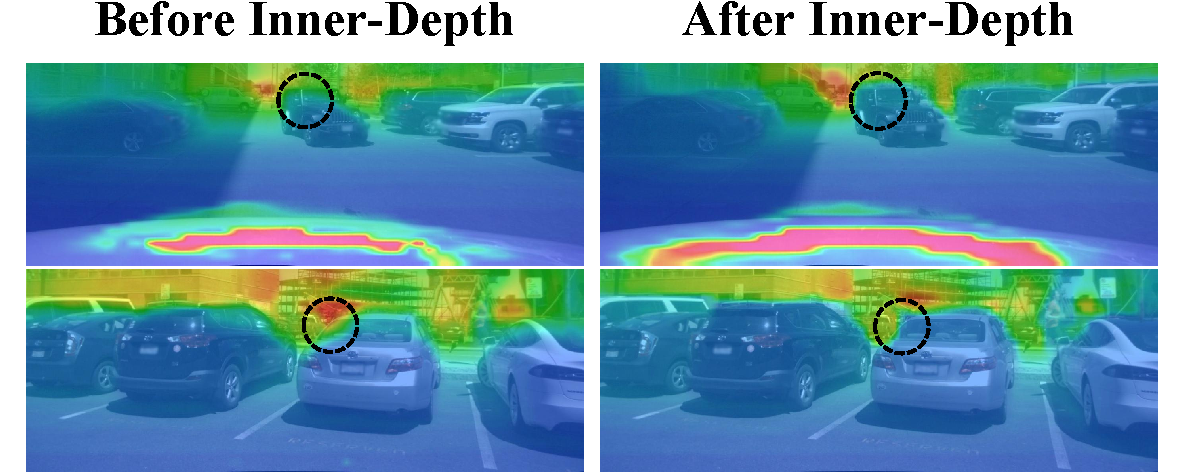
\includegraphics[scale=0.4]{cvpr_2022/ref_vis.pdf}
    \caption{\textbf{Visualization of Predicted Depth Maps,} which are before and after the inner-depth supervision, respectively.}
    \label{fig:ref_compare}
    %\hspace{-5cm}
\end{figure}

\paragraph{Inner-geometry Learning.} 
%\KY{find a better name}
The individual effectiveness of the two main components can be examined by only equipping one of them. We first study the impact of the inner-depth supervision. As shown in Table~\ref{tab:main_ablation}, we only introduce the inner-depth supervision to the vanilla baseline, i.e., BEVDepth, by which its mAP improves from 32.9\% to 33.9\% with a +1.0\% gain and its NDS reaches 44.0\% from 43.1\% with a +0.9\% gain. 
Instead, when we only use the inner-feature BEV distillation, the mAP boosts from 32.9\% to 35.9\% with a +3.0\% improvement and the NDS boosts from 43.1\% to 45.4\% with a +2.3\% improvement. In addition, the combination of both components achieves better +3.7\% mAP and +2.7\% NDS, demonstrating that the two proposed objectives might be complementary.

%\begin{figure} [t]
%    \centering 
%    \subfloat[\label{fig:a}]{
%		\includegraphics[scale=0.13]{cvpr_2022/relative_vis_before.png}}
%    \subfloat[\label{fig:b}]{
%		\includegraphics[scale=0.13]{cvpr_2022/relative_vis_after.png}}
%    \vspace{-3mm}
%    \caption{\textbf{The visualization of depth distribution.} (a) shows the origin predicted depth distribution of each valid pixel where exists projectable lidar points, while the depth distribution in (b) is predicted after inner relative depth supervision. The horizontal axis represents the discrete depth $\mathcal{D}_{\rm{i}}$ within the range of $\mathcal{[}0\mathcal{,}\mathcal{D}_{\rm{max}}\mathcal{]}$. The yellow pillar refers to the ground truth of depth and the red pillar refers to the predict depth whose height indicates the probability of the corresponding depth. The most obvious difference is marked in blue boxes.} 
%    \label{fig:imgnet_sigma} 
%    \vspace{-3mm}
%\end{figure}





%\begin{table}[t!]
%    \centering
%    \caption{\textbf{Ablation Study of Distillation.}  }
%    \vspace{-2mm}
%    \resizebox{1\columnwidth}{!}
%    {\tablestyle{20pt}{0.8}
%    \begin{tabular}{c|c|c}
%    \toprule
%          Methods& mAP&NDS  \\
%          \midrule
%                        Dense Feature Mimic  & 0.338         & 0.434 \\ 
%             Soft Foreground Feature Mimic  & 0.328        & 0.427 \\
%             Ours & \textbf{0.366}         & \textbf{0.458} \\
%    \bottomrule
%    \end{tabular}}
%    \label{tab:distill_ablation}
%    \vspace{-3mm}
%\end{table}


%We are also interested in that if the learning target (\ie teacher feature) is fixed, can the student adapt itself through target-aware transformer better? We compare different settings of $\theta(\cdot)$ including identical mapping against Conv$+$BN. The result on Cifar100 is presented on Table \ref{tab:cifar_1x1}. Surprisingly, the identical mapping for $\theta(\cdot)$ always performs better. 

%We further investigate the non-parametric implementation by setting both $\theta(\cdot)$ and $\gamma(\cdot)$ as identical mapping on ImageNet (Table~\ref{tab:non-parametric_imagenet}). The result shows that the semi-parametric version performs best, where the fixed teacher and the linear transformation applying to student feature can facilitate the student to reconfigure itself.



\begin{table}[t!]
    \centering
    \caption{\textbf{Ablation Study of Inner-feature BEV Distillation.} $\mathcal{L}^{IC}_{\rm{bev}}$ and $\mathcal{L}^{IK}_{\rm{bev}}$ denote the losses of inter-channel and inter-keypoint distillation, respectively.}
    %\vspace{-2mm}
    \resizebox{1\columnwidth}{!}
    {\tablestyle{15pt}{1.0}
    \begin{tabular}{cc|cc}
    \toprule[1.2pt]
          $\mathcal{L}^{IC}_{\rm{bev}}$&$\mathcal{L}^{IK}_{\rm{bev}}$& mAP&NDS  \\
          \midrule
                        &           & 0.329         & 0.431 \\ 
             \checkmark &           & 0.342         & 0.444 \\
                        &\checkmark & 0.358         & 0.452 \\
              \checkmark&\checkmark & \textbf{0.366}         & \textbf{0.461} \\
    \bottomrule[1.2pt]
    \end{tabular}}
    \label{tab:saf_ablation}
    %\vspace{-3mm}
\end{table}

\paragraph{Inner-depth Supervision.}
To calculate the relative depth values within foreground targets, we compare several methods concerning the relationships among different inner points, which can be divided into three paradigms, 1) \emph{All-to-Certain} calculates the relative depth from all sampled points to a certain reference point, such as the projected center of 3D bounding box or the center of 2D bounding box. 2) \emph{All-to-Adaptive} sets the reference depth in a dynamic manner, which selects the reference pixel with the highest confidence across all depth bins or the smallest depth error to the ground truth (Ours). 3) \emph{One-to-One} calculates the relative depth from each two sampled point pair. As shown in Table~\ref{tab:relative_ablation}, compared with other patterns, our \emph{All-to-Adaptive} with smallest depth errors obtains the best performance improvement, which indicates the dynamic depth reference point can flexibly adapt to different targets for inner-geometry learning. What's more, we visualize our depth prediction with and without the inner-depth supervision in Figure~\ref{fig:ref_compare}, which effectively refines the contours and edges of foreground objects.


\paragraph{Inner-feature BEV Distillation.}
Our TiG-BEV explores the BEV feature distillation from two perspectives, inter-channel and inter-keypoint. To validate their effectiveness, we also equip the model with one of them at a time and report the results in Table~\ref{tab:saf_ablation}. As shown, both inter-channel and inter-keypoint distillation contribute to the final performance, respectively boosting the NDS by +1.3\% and +2.1\%. This well illustrates the importance of learning inner-geometry semantics within different foreground targets in BEV space. Further combining them two can benefit the performance by +3.7\% and +3.0\% for mAP and NDS.

\paragraph{2D Backbones and Temporal Information.}
We further explore the influence of 2D backbones and temporal information to our TiG-BEV in Table~\ref{tab:many_ablation}. We observe that our TiG-BEV brings significant performance improvement consistent over different 2D backbones. Also, our target inner-geometry learning schemes can provide positive effect for both single-frame and multi-frame settings. The improvement of mAP ranges from \textbf{+3.4\%} to \textbf{+5.8\%} and the improvement of NDS ranges from \textbf{+2.5\%} to \textbf{+5.0\%}.



%We also conduct the thorough experiments to understand the contribution brought by the proposed patch-group distillation $\mathcal{L}_{\rm{TaT}}^{\mathcal{P}}$ and anchor-point distillation $\mathcal{L}_{\rm{TaT}}^{\mathcal{A}}$. As discussed previously, $\mathcal{L}_{\rm{TaT}}^{\mathcal{A}}$ is proposed to learn the global representation to capture long-range dependency while $\mathcal{L}_{\rm{TaT}}^{\mathcal{P}}$ is designed to concentrate on local feature. 
%By covering each one of them, the individual effectiveness of the two components can be examined.  
%As shown in Table. \ref{tab:main_ablation}, both objectives can improve the vanilla student significantly while $\mathcal{L}_{\rm{TaT}}^{\mathcal{P}}$ presents more efficacy. 
%The combination of both components achieves the best performance, demonstrating that the two proposed objectives are complementary.  

% Then, we give more insight with respect to the proposed objectives' functionality through sensitivity analysis. Specifically, we investigate the hyper-parameters that would influence the behaviour of the training process. In terms of the anchor-point distillation, this work utilizes average pooling to extract the anchor in a local area from the original feature, forming the associated anchor-point feature. It is a trade-off between noise reduction and representation preservation since bigger kernel would filter more noise along with more informative representation. Thus we study the sampling range (i.e. kernel size) that directly yields different feature resolution. Specially, when the $1\times 1$ pooling kernel is used, it degrades to the circumstance discussed in Sec. \ref{sec:formulation} and returns the original feature.
% The result exhibited in Table \ref{tab:anchor} supports our hypothesis that the full-size feature deteriorates the performance due to noise interference and presents poor performance compared to the other anchor-point features of smaller size. On the other hand, excessive sampling range would omit useful and informative representation and damage the performance.



% \mypara{Extra Width.}
% Then, we give more insight concerning the proposed extra width's functionality through ablation study. Specifically, we suppose that introducing extra width for ground truth bounding box before grid sampling would allow the distillation process to focus more on the edge information of foreground objects. 



%So we varied the value of the extra width by 0, 1, 2, 3 unit while keeping the other variables consistent, the length of an unit is equal to the width of a bev grid. 
%It is a trade-off between reducing computation overhead and summarizing fine-grained spatial information since a bigger kernel would reduce feature size along with more informative representation, \eg, when feature map size is reduced to $1 \times 1$, it degrades to ignoring the spatial information and posing one-to-one fashion distillation.
%Thus we study the pooling kernel size that directly yields different feature resolutions.
% Especially, when the $1\times 1$ pooling kernel is used, it degrades to the circumstance discussed in Section \ref{sec:formulation} and returns the original feature.
%The result exhibited in Table \ref{tab:anchor} supports our hypothesis that the full-size feature deteriorates the performance due to inferior capacity of student network and presents poor performance compared to the other anchor-point features of smaller size. On the other hand, excessive sampling range would omit useful and informative representation and damage the performance.
% The result exhibited in Table \ref{tab:comb_ablation} shows that when the extra width exists, our approach can further enhance the mAP. 

%Next we analyze the roi grid size used in grid sampling, the key factor of our inner-feature bev distillation.In Table \ref{tab:comb_ablation}, we found that generally, larger grid size is advantageous to our distillation, however we should make a trade-off because of the decreasing marginal gains. Overall, we found that the combination of $24\times 24$ grid size and using extra width can reach the best performance.
%however overlarge grid size may be unfavourable and we should make a trade-off between reducing computation overhead and extracting fine-grained spatial information since a $N\times N$ grid size results in $(N\times N)\times(N\times N)$ feature supervision. In our ablation study, we found that the combination of $24\times 24$ grid size and 2 unit extra width can reach the best performance.
%On the other hand, excessive extra width would lead to inadequate foreground structure supervision which will damage the performance.
%\begin{table}[t!]
%    \centering
%    \caption{\textbf{Ablation Study of Extra Width.} }
%    \vspace{-3mm}
%    \resizebox{1\columnwidth}{!}
%    {\tablestyle{10pt}{1}
%    \begin{tabular}{@{}l|ccccc@{}} 
%    \toprule
%         Extra width &0 &1 &2 &3    \\
%         \midrule
%         mAP &0.326 &\textbf{0.336} &0.335 &0.331\\
%         NDS &0.369 &\textbf{0.372} &0.364 &0.363 \\
%    \bottomrule
%    \end{tabular}
%    \label{tab:extra_width}}
%\vspace{-3mm}
%\end{table}

%\begin{table}[t!]
%    \centering
%    \caption{\textbf{Ablation Study of ROI Grid Size.}}
%    \vspace{-3mm}
%    \resizebox{1\columnwidth}{!}
%    {\tablestyle{10pt}{1}
%    \begin{tabular}{@{}l|cccc@{}}
%    \toprule
%         Grid size &$8\times 8$ &$16\times 16$&$24\times 24$&$32\times 32$ \\
%         \midrule
%        mAP &0.331 &0.335   &\textbf{0.338} & 0.333 \\
%        NDS &0.357 &0.364   &\textbf{0.375} & 0.354 \\
%    \bottomrule
%    \end{tabular}
%    \label{tab:grid_size}}
%    \vspace{-3mm}
%\end{table}








%\mypara{Ablation Study of ROI Grid Size.}
%Next we analyze a key factor of our structured attention feature supervision, the roi grid size used in grid sampling. In Table \ref{tab:comb_ablation}, we found that generally, larger grid size is advantageous to our distillation, however overlarge grid size may be unfavourable and we should make a trade-off between reducing computation overhead and extracting fine-grained spatial information since a $N\times N$ grid size results in $(N\times N)\times(N\times N)$ feature supervision. In our ablation study, we found that the combination of $24\times 24$ grid size and 2 unit extra width can reach the best performance.



% \begin{table}[t!]
% \centering
%     \caption{\textbf{Ablation Study of Extra Width.}}
%     %\vspace{-2mm}
%     \resizebox{1\columnwidth}{!}
%     {\tablestyle{25pt}{1.0}
%     \begin{tabular}{c|c|c}
%     \toprule[1.2pt]
%           Extra Width&mAP&NDS  \\
%           \midrule
%           &0.360       &  0.457     \\
%           %\midrule
%           \checkmark&  \textbf{0.366}      & \textbf{0.461}      \\
              
%     \bottomrule[1.2pt]
%     \end{tabular}}
%     \label{tab:comb_ablation}
%     %\vspace{-5mm}
% \end{table}

\iffalse
\begin{table}[t!]
\centering
    \caption{\textbf{Ablation Study of Different Combination of Extra Width and Grid Size.}}
    %\vspace{-2mm}
    \resizebox{1\columnwidth}{!}
    {\tablestyle{25pt}{0.8}
    \begin{tabular}{c|c|c|c}
    \toprule[1.2pt]
          Extra Width&Grid Size&mAP&NDS  \\
          \midrule
          \multirow{3}{*}{}&$16\times 16$ & 0.359       &  0.459     \\
                                      &$24\times 24$ & 0.360       &  0.457     \\
                                      &$32\times 32$ & 0.361       &  0.458     \\
          \midrule
          \multirow{3}{*}{\checkmark}&$16\times 16$ & 0.362       & 0.458      \\
                                      &$24\times 24$ &  \textbf{0.366}      & \textbf{0.461}      \\
                                      &$32\times 32$ &  0.365      &  0.458     \\
              
    \bottomrule[1.2pt]
    \end{tabular}}
    \label{tab:comb_ablation}
    %\vspace{-5mm}
\end{table}
\fi


\iffalse
\begin{table}[t!]
\centering
    \caption{\textbf{Ablation Study of Different Combination of Extra Width and Grid Size.}}
    %\vspace{-2mm}
    \resizebox{1\columnwidth}{!}
    {\tablestyle{20pt}{0.8}
    \begin{tabular}{c|c|c|c}
    \toprule[1.2pt]
          Extra Width&Grid Size&mAP&NDS  \\
          \midrule
          \multirow{4}{*}{0}&$8\times 8$ & \textbf{0.333}  & \textbf{0.377} \\ 
                                      &$16\times 16$ & 0.326       &  0.369     \\
                                      &$24\times 24$ & 0.330       &  0.352     \\
                                      &$32\times 32$ & 0.325       &  0.350     \\
          \midrule
          \multirow{4}{*}{1}&$8\times 8$ & 0.334  & 0.363 \\ 
                                      &$16\times 16$ &  \textbf{0.336}      &  \textbf{0.372}     \\
                                      &$24\times 24$ &  0.335      &  0.364     \\
                                      &$32\times 32$ &  0.333      &  0.353     \\
          \midrule
          \multirow{4}{*}{2}&$8\times 8$ & 0.331  & 0.357 \\ 
                                      &$16\times 16$ & 0.335       & 0.364      \\
                                      &$24\times 24$ &  \textbf{0.338}      & \textbf{0.375}      \\
                                      &$32\times 32$ &  0.333      &  0.354     \\
          \midrule
          \multirow{4}{*}{3}&$8\times 8$ & 0.331 &0.357  \\ 
                                      &$16\times 16$ & 0.331       &  \textbf{0.363}     \\
                                      &$24\times 24$ & 0.333  & 0.361  \\
                                      &$32\times 32$ & \textbf{0.335}       &  0.358     \\

              
    \bottomrule[1.2pt]
    \end{tabular}}
    \label{tab:comb_ablation}
    %\vspace{-5mm}
\end{table}
\fi

